\documentclass[a4paper,12pt,twoside]{report}%pridat twoside, do [] pre obojstrannu tlac
\pagestyle{headings}
\linespread{1.5} % riadkovanie
\usepackage[top=2.5cm, bottom=2.5cm, left=3.5cm, right=2cm]{geometry} %odporucane okraje
%    \usepackage[top=2.9cm, bottom=2.9cm, left=2.5cm, right=4cm]{geometry} %okraje
%\evensidemargin=-0cm       %uprava okrajov
%\oddsidemargin=+1.5cm        %uprava okrajov

%nieco od Jakuba:
\pdfpagewidth=\paperwidth                        % zabezpecuje, aby to v~pdf malo rovnaky rozmer ako v~dvi,
\pdfpageheight=\paperheight                      % tie za beznych okolnosti nemusia moc dobre korelovat

%English, slovak
\usepackage[utf8x]{inputenc}
\usepackage[slovak,english]{babel}%ked je opacne poradie, bude "Obsah" namiesto "Contents" a podobne
%\usepackage{palatino,verbatim} %ine pismo

%male popisy obrazkov a~grafika
\usepackage[font=small,margin=0.5cm]{caption} % margin reguluje okraje popisu obrazka (v pripade, ze je na sirku strany a~ma viac ako 1 riadok)
\usepackage[dvips]{graphicx}
\usepackage{wrapfig}
\usepackage[usenames,dvipsnames]{color}
\usepackage{epstopdf}   %bez tohto pdflatex nezoberie eps obazky

%grid obrazkov
\usepackage{subfig}

\newcounter{eqn}
\renewcommand*{\theeqn}{\alph{eqn})}
\newcommand{\num}{\refstepcounter{eqn}\text{\theeqn}\;}

%farebne tabulky
\usepackage{colortbl}
\usepackage[table]{xcolor}
%na otacanie tabuliek
\usepackage{rotating}

%odsadenie prveho odstavca
\usepackage{indentfirst}

%Matematicke vyrazy
\usepackage{amsfonts}
%\usepackage{amsmath}
\usepackage{amssymb}
\usepackage[intlimits]{amsmath}

\usepackage{verbatim}
\usepackage{url}

%definicie
\newcommand{\p}{\partial}
\def\epsilon{\varepsilon}
\def\Bf#1{\mathbf{#1}}

%ani neviem co je toto
\makeatletter
\newenvironment{tablehere}
{\def\@captype{table}}
{}

\author{Gerg\H{o} Ibolya}
\title{Numerical solution of the 1D viscous Burgers' and traffic flow equations by the inflow-implicit/outflow-explicit finite volume method}

%Hyperreferencia
\usepackage{hyperref}
\hypersetup{colorlinks,citecolor=black,filecolor=black,linkcolor=black,urlcolor=black,pdftex}

%figure drawing
%\usepackage{graphicx,subcaption}
\usepackage{tikz,tikz-3dplot}
\usepackage{float}
\usepackage{color}

%====================================================================================================================================================
%====================================================================================================================================================

\begin{document}
	\setlength{\belowdisplayskip}{7pt} \setlength{\belowdisplayshortskip}{5pt} \setlength{\abovedisplayskip}{7pt}
	\setlength{\abovedisplayshortskip}{5pt}
	
	%***********************zaciatok prvej strany
	\thispagestyle{empty}
	{
		\topmargin=0pt
		\centerline {\large \bf{SLOVAK UNIVERSITY OF TECHNOLOGY IN BRATISLAVA}}
		\vskip 0.2cm
		\centerline{\large \bf{FACULTY OF CIVIL ENGINEERING}}
		\vskip 5cm
		\centerline{\Large \bf{Numerical solution of nonlinear advection equations by the}}
		\vskip 0.2cm
		\centerline{\Large \bf{inflow-implicit/outflow-explicit finite volume method}}
		%\centerline{ \bf{(verzia z~\today) }}   %vypisovanie dnesneho datumu
		\vskip 0.5cm
		\centerline{\large \bf{Project of PhD thesis}}
		\vskip 5cm          %\vskip 2cm             %zmena kvoli zobrazovaniu dnesneho datumu
		\normalsize
		\begin{tabular}[l]{p{0.27\textwidth}p{0.73\textwidth}}
			Field of study: & Applied mathematics\\
			Department: & Department of Mathematics and Descriptive Geometry\\
			Supervisor: & prof. RNDr. Karol Mikula, DrSc. \\
		\end{tabular}
		\vskip 3cm
		\centerline{\large \bf{BRATISLAVA 2021}}
		\vskip 0.2cm
		\selectlanguage{slovak}
		\centerline{\large \bf{Ing. Gerg\H{o} Ibolya}}
		\selectlanguage{english}
	}
	\pagebreak
	%**********************************koniec prvej strany
	%prazdna strana
	%\newpage
	%\thispagestyle{empty}
	%\mbox{}
	%\newpage
	%====================================================================================================================================================
	
	\mbox{}
	\vfill
	\thispagestyle{empty}
	\section*{Acknowledgement}
	I want to thank my thesis supervisor prof. RNDr. Karol Mikula, DrSc. for the help, dedicated time during consultations, expert guidance and valuable advices in the elaboration of this thesis. This work was supported by the grants  APVV-19-0460, VEGA 1/0709/19 and VEGA 1/0436/20.
	\newpage
	
	
	\thispagestyle{empty}
	\mbox{}
	\newpage
	
	\section*{Abstract}
	\thispagestyle{empty}
In our work we present a numerical solution of equations arising from continuum fluid and traffic flow models by the inflow-implicit/outflow-explicit(IIOE) method. The method is based on finite volume space discretization and a semi-implicit discretization in time. It has a formal second order accuracy. Inflows to the cells are treated implicitly and outflows explicitly. Comparisons of numerical solutions with the exact ones are presented. 
	\newline\newline
	
	\textbf{Keywords: viscous Burgers' equation,  traffic flow, nonlinear conservation laws, finite volume method, semi-implicit scheme}
	\newpage
	%====================================================================================================================================================
{\pagestyle{headings}
	\tableofcontents
	\cleardoublepage}

%====================================================================================================================================================

\chapter{Introduction}\label{introduction}%Preface?
\chaptermark{Introduction}
The three dimensional Navier-Stokes equations for incompressible flow:
\begin{align}
	u_t + u u_x + v u_y + w u_z &= - \frac{p_x}{\rho} + \sigma (u_{xx} + u_{yy} + u_{zz})\nonumber \\
	v_t + u v_x + v v_y + w v_z &= - \frac{p_y}{\rho} + \sigma (v_{xx} + v_{yy} + v_{zz}) \label{navier-stokes} \\
	w_t + u w_x + v w_y + w w_z &= - \frac{p_z}{\rho} + \sigma (w_{xx} + w_{yy} + w_{zz})\nonumber \\
	u_x + v_y + w_z &= 0\nonumber,
\end{align}
where $ u, v, w $ are the components of the velocity vector in the directions of coordinate axes $ x, y, z $ respectively, $ p $ is the pressure, $ \sigma \geq 0 $ denotes kinematic viscosity. The first three equations can be derived from Newton's second law of conservation of linear momentum in Eulerian description of fluid motion. It says that the acceleration of an infinitesimally small volume of fluid is proportional to the net force acting on it and inversely proportional to its mass. The fourth equation says that the fluid is incompressible, i.e. the veloctiy field is divergence free.
\par These equations can be solved analytically only in a few simple cases. However, it is of practical and theoretical interest to solve the complicated equations without much simplifications. The trouble is mainly caused by the nonlinear advective acceleration terms in the conservation of linear momentum equations.
\section{Burgers' equation}

Considering that only the $ u $ component of the velocity field is nonzero and it is a function of $ x $ only, neglecting the pressure term we get from \eqref{navier-stokes} the one dimensional viscous Burgers' equation 
\begin{equation}
u_t + uu_x = \sigma u_{xx},
\label{burg}
\end{equation}
named after a Dutch physicist Johannes Martinus Burgers, \cite{burgers}. It is interesting to note that the equation was first studied by a British (later American) applied matematician Harry Bateman, \cite{bateman}.
The equation captures some  key features of the equations of fluid dynamics: nonlinear advection, arising from the advective acceleration terms in the conservation of linear momentum equations, and viscosity \cite{lev}. The equation can be solved analytically by transforming it to the linear heat equation, known as the Cole-Hopf transformation \cite{olv, whitham}. This fact allows us to compare numerical solutions with the exact one. By studying the behaviour of its numerical solutions, we can predict the performance of a particular numerical scheme on the more complicated equations of fluid dynamics.

\section{Traffic flow}

Similiar equation describes the change of the density of cars in continuum traffic-flow models. Let us give a brief description of one of the simplest and oldest such model, known as the LWR model after Lighthill, Whitham \cite{lighthillwitham} and Richards \cite{richards}, whence the name. First assume that the cars are smoothly distributed on a one-lane highway so we can define a continous function of the density $ \rho (t,x) $ given in number of cars/unit length. Then the conservation of cars states that without any sources or sinks
\begin{center}
	the change of the number of cars = incoming cars - outgoing cars.
\end{center}
We can define the flux of cars as $ f(\rho) = \rho v(\rho) $, where $ v(\rho) $  denotes the speed in the direction of $ x $ axis in units distance(given in unit length)/time, which we assume is a non-increasing function of the density. It is reasonable to expect that a car is moving slower in a denser traffic. In other words, the speed of a car decreases as the density increases. It is easily seen that the flux function defined above has units number of cars/time, as it should be. Mathematically we can write the conservation law on a given section of the lane $ \left[x_1, x_2\right] $ and in a given time interval $ [t_1, t_2] $ as follows:
\[
\int_{x_1}^{x_2} \rho (t_2,x) \mathrm{d}x - \rho (t_1,x)\,\mathrm{d}x = \int_{t_1}^{t_2} f(\rho(t,x_1)) - f\left(\rho(t,x_2)\right)\mathrm{d}t.
\]
Assuming that the functions are smooth and continously differentiable on the given intervals, using the Newton-Leibniz theorem we can rewrite the law as
\[
\int_{x_1}^{x_2} \int_{t_1}^{t_2} \frac{\partial}{\partial t}\rho(t,x) \,\mathrm{d}t\, \mathrm{d}x = -\int_{t_1}^{t_2} \int_{x_1}^{x_2} \frac{\partial}{\partial x} f\left(\rho(t,x)\right)\, \mathrm{d}x\, \mathrm{d}t.
\]
The intervals can be arbitrarily chosen, this leads us to the differential form of the conservation of cars:
\begin{equation}
	\rho_t + f(\rho)_x = 0
	\label{conservation}
\end{equation}
%\begin{equation}
%	\begin{cases}
%		\rho_t + f(\rho)_x=0 & x\in \mathbb{R},\, t > 0\\
%		\rho (0,x) = \rho_0(x) & x\in \mathbb{R}
%	\end{cases}
%\end{equation}
One simple example, known as the Greenshield's model \cite{greenshields}, who proposed a linear relationship between the density and velocity
\[
v(\rho) = 1-\rho.
\]
Here we simply assume that the units are chosen in an appropriate way to have $ 0 \leq \rho \leq 1 $ and also $ 0 \leq v(\rho) \leq 1 $. For example, the density can be measured in units of cars/car length, for simplicity assuming that every car has the same length. Then $ \rho = 1 $ and $ \rho = 0 $ represents bumper to bumper traffic and empty road respectively.
These assumptions lead to a nonlinear flux function
\[
f(\rho) = \rho \left(1 - \rho \right) 
\]
A way to extend this model, is to assume that the flux also depends on the density gradient. If the traffic is getting denser more rapidly the drivers are reducing their speed more. Applying this yields a modified flux function
\begin{equation}
	f(\rho, \rho_x) = \rho \left(1 - \rho\right) - D \rho_x,
	\label{flux}
\end{equation}
where $ D $ is a diffusion coefficient. Substituting (\ref{flux}) to (\ref{conservation}) and putting the diffusion term to the right-hand side we get
\begin{equation}
	\rho_t + u(\rho)\rho_x = D \rho_{xx},
	\label{traffic}
\end{equation}
where we denoted
\begin{equation}
	u(\rho) = 1 - 2\rho.
	\label{u-ro}
\end{equation}
Multiplying both sides by $ u'(\rho) $ we obtain
\[ u'(\rho)\rho_t + u(\rho)u'(\rho)\rho_x = D u'(\rho)\rho_{xx},\]
which can be rewritten as
\[ u_t + uu_x = D u_{xx} - D u''(\rho) \rho_x^2. \]
Since $ u''(\rho) = 0 $ we end up with the viscous Burgers' equation (\ref{burg}), where $ \sigma $ corresponds to the diffusion coefficient $ D $. By solving (\ref{burg}) and using the relationship (\ref{u-ro}) we easily obtain a relation for the density
\begin{equation}
	\rho(u) = \frac{1}{2}\left(1 - u\right).
	\label{ro-u}
\end{equation}
The model discussed above is a simple first order continuum model of the traffic. Since its first appearence several other higher order models have been developed with more or less success.
However, despite its deficiencies, it can give us valuable insight into how cars are behaving in a traffic.

%====================================================================================================================================================
\chapter{Inflow-implicit\slash outflow-explicit method\label{worksummary}}
\chaptermark{Inflow-implicit\slash outflow-explicit}

\par There is only a relatively small number of cases, when we can find an analytical solution for a differential equation. Therefore the development of numerical methods for finding approximate solutions with the desired accuracy is very important. For solving partial differential equations, several numerical methods have been developed. Among the most popular numerical techniques are the finite difference method, the finite volume method and the finite element method. These methods reduce the problem of solving a differential equation to a solution of a system of equations. Below we give a brief description of these methods for the 1D case, which is relevant to this work.

The finite difference method is the oldest and in some ways the simplest approach. The idea is to replace  differentiation in the equation with differences. The domain of interest is divided into a given number of elements. The differences are calculated from the approximate values at the nodes. The way, in which we calculate the differences are from accuracy and stability considerations.

The finite volume method uses a different approach. First we subdivide our spatial domain of interest into "finite volumes" or grid cells. In 1D these are intervals on the real line. We denote the $ i $-th grid cell by
\[
p_i = (x_{i-1/2}, x_{i+1/2})
\]
with length.
The method is based on the conservation of a quantity $ u(t, x) $. Instead of looking for approximations of the values of $ u $ at the nodes, as we do in the finite difference method, we are interested in the approximations of the integral of $ u $ over each interval. The change of the integral over a time interval $ [t^{n}, t^{n+1}] $ is due to the fluxes $ f(t, x) $ at the endpoints of the cells:
\[
\int_{p_i} u(t^{n+1}, x) \,\mathrm{d}x - \int_{p_i} u(t^{n}, x) \,\mathrm{d}x = 
\int_{t^{n}}^{t^{n+1}} f(t, x_{i-1/2}) \,\mathrm{d}t - \int_{t^{n}}^{t^{n+1}} f(t, x_{i+1/2}) \,\mathrm{d}t.
\]
Our goal is to calculate how the integral changes over time, i.e. if we know the integral at time $ t^n $, what is its value at a later time $ t^{n+1} $.
For this purpose we approximate the average value of $ u $ by a constant represantative value denoted as $ \bar{u}_i^n $ inside the $ i $-th cell at time $ t^n $. The approximation of the integral becomes
\[
\int_{p_i} u(t^n, x) \,\mathrm{d}x \approx \bar{u}_i^n h,
\]
where  $ h = x_{i+1/2} - x_{i-1/2} $ is the length of a cell.
We can also express
\[
\int_{t^{n}}^{t^{n+1}} f(t, x_{i-1/2}) \,\mathrm{d}t \approx f_{i-1/2} \tau,
\]
where $ f(t, x_{i-1/2}) $ is an approximation to the average flux at $ x_{i-1/2} $ and $ \tau = t^{n+1} - t^n $.
After substitution the conservation law takes the form
\[
\bar{u}_i^{n+1} h - \bar{u}_i^n h = f_{i-1/2} \tau -  f_{i+1/2} \tau
\]
Dividing by the length of the cell $ h $, rearranging terms we get an expression for the average value at time $ t^{n+1} $ as
\[
\bar{u}_i^{n+1} = \bar{u}_i^n - \frac{\tau}{h}(f_{i+1/2} - f_{i-1/2}).
\]
If we approximate the average fluxes using the constant representative values $ \bar{u}_i^{n} $ we get a fully discrete method.

The finite element method is based either on a minimization principle, if possible, or on the concept of a weak solution to a differential equation. 

 For problems, where solutions are tending to develop shock waves, the discontinous Galerkin method became very popular.
\par In this work we apply the inflow-implicit\slash outflow-explicit (IIOE) scheme  to the nonlinear advection term of equation (\ref{burg}). The method is based on finite volume space discretization and a semi-implicit discretization in time. Inflows to the cells are treated implicitly and outflows are treated explicitly. We could explain this idea intuitively that we know what is flowing out from a cell at a given time but leave the method to solve a system of equations determined by the inflows to obtain the solution values at the new time step. The IIOE scheme is formally second order accurate in space and time for 1D advection problems with variable velocity \cite{iioe2}. Combining with the Crank-Nicolson scheme for the diffusion term, we get a new numerical scheme for the nonlinear advection-diffusion problem (\ref{burg}) considered in this article.
%====================================================================================================================================================

\section{Numerical scheme}
For reader convenience we present here the derivation of the IIOE scheme \cite{iioe0,iioe1,iioe2} for the equation
\begin{equation}
	u_t + vu_x = 0, 
	\label{adv}
\end{equation}
where $ v = v(x) $. We rewrite (\ref{adv}) in the equivalent form
\begin{equation}
	u_t + (vu)_x - uv_x = 0,
	\label{adv1}
\end{equation}
and integrating over a grid cell $ p_i $ with cell center $ x_i $, length $ h $, left border $ x_{i-\frac{1}{2}} $, right border $ x_{i+\frac{1}{2}} $ yields
\[ \int_{p_i} u_t\, dx + 
\int_{p_i}(vu)_x\, dx - 
\int_{p_i} uv_x\, dx = 0\]
Let us denote $ v_i = v(x_i) $, $ v_{i - \frac{1}{2}} = v(x_{i-\frac{1}{2}}) $, $ v_{i + \frac{1}{2}} = v(x_{i+\frac{1}{2}}) $. Let us denote by $ u_i^n $ a constant value of the solution inside the $ i $-th finite volume cell at time step $ n $ computed by the numerical scheme. We use a constant representation of the solution inside a cell $ p_i $ denoted by $ \bar u_i $ and constant representative values at the cell interfaces denoted by $ \bar u_{i - \frac{1}{2}} $, $ \bar u_{i + \frac{1}{2}} $ respectively. Using the Newton-Leibniz formula we obtain
\[ \int_{p_i} u_t\, dx +
v_{i + \frac{1}{2}} \bar u_{i + \frac{1}{2}} - v_{i - \frac{1}{2}} \bar u_{i - \frac{1}{2}} - 
\bar u_i (v_{i + \frac{1}{2}} - v_{i - \frac{1}{2}}) = 0. \]
By rearranging terms we get
\[\int_{p_i} u_t\, dx + 
v_{i - \frac{1}{2}}(\bar u_i - \bar u_{i - \frac{1}{2}}) + (-v_{i + \frac{1}{2}})(\bar u_i - \bar u_{i + \frac{1}{2}}) = 0.\]
$ v_{i - \frac{1}{2}} > 0 $ represents inflow from the left cell interface, while $ (-v_{i + \frac{1}{2}}) > 0 $ represents inflow from the right cell interface. Otherwise they represent outflows. Thus we define
\begin{eqnarray*}
	a^{in}_{i-\frac{1}{2}} = \textrm{max}(v_{i-\frac{1}{2}},0),\quad 
	a^{out}_{i-\frac{1}{2}} = \textrm{min}(v_{i-\frac{1}{2}},0), 
	\\
	a^{in}_{i+\frac{1}{2}} = \textrm{max}(-v_{i+\frac{1}{2}},0),\quad 
	a^{out}_{i+\frac{1}{2}} = \textrm{min}(-v_{i+\frac{1}{2}},0). 
\end{eqnarray*}
We use a simple finite difference approximation for the time derivative $ \frac{u^n_i - u^{n-1}_i}{\tau} $,
where $ \tau $ is a uniform time step, take inflow implicitly, outflow explicitly and use the straightforward reconstructions $ \bar u_i^n = u^n_i $, $ \bar u_{i - \frac{1}{2}}^n = \frac{1}{2} (u_i^n + u_{i-1}^n) $, $ \bar u_{i + \frac{1}{2}}^n = \frac{1}{2} (u_i^n + u_{i+1}^n) $, we obtain the basic one-dimensional IIOE scheme for variable velocity:
\begin{eqnarray}
	\label{iioe0}
	u^n_i + \frac{\tau}{2h} a^{in}_{i-\frac{1}{2}}  \left(u^n_i - u^n_{i-1}\right) + 
	\frac{\tau}{2h} a^{in}_{i+\frac{1}{2}} \left(u^n_i - u^n_{i+1}\right) = \\
	u^{n-1}_i - \frac{\tau}{2h} \left(a^{out}_{i-\frac{1}{2}} \left(u^{n-1}_i - u^{n-1}_{i-1}\right) + 
	a^{out}_{i+\frac{1}{2}} \left(u^{n-1}_i - u^{n-1}_{i+1}\right)\right).\nonumber
\end{eqnarray}
For the advective part of the Burgers' equation (\ref{burg}) we calculate the velocities from the solution at the cell interfaces, for which we use the same reconstructions as before. This leads us to a nonlinear system of equations, which we solve iteratively. The time dependent velocities in the $ k $-th iteration become
\[ v^{n,k}_{i-\frac{1}{2}} = (u^{n,k-1}_i + u^{n,k-1}_{i-1})\slash 2,\quad
v^{n,k}_{i+\frac{1}{2}} = (u^{n,k-1}_i + u^{n,k-1}_{i+1})\slash 2,\quad k=1,2,3,.... \]
and $ u^{n,0}_i = u^{n-1}_i $.

When solving the traffic flow problem (\ref{traffic}), we replace $ u^n_i $ by $ \rho^n_i $. Considering that characteristic speed in the equations of traffic flow \eqref{traffic} equals $ 1-2\rho $, using the same reconstructions as for $ u^n_i $ and cancelling common factors, the time dependent velocities according to (\ref{u-ro}) in the $ k $-th iteration become
\[ v^{n,k}_{i-\frac{1}{2}} = 1 - (\rho^{n,k-1}_i + \rho^{n,k-1}_{i-1}),\quad
v^{n,k}_{i+\frac{1}{2}} = 1 - (\rho^{n,k-1}_i + \rho^{n,k-1}_{i+1}). \]
In both cases we consider the time dependent splitting to inflows and outflows
\begin{eqnarray}
	a^{in,n,k}_{i-\frac{1}{2}} = \textrm{max}(v^{n,k}_{i-\frac{1}{2}},0),\quad 
	a^{out,n}_{i-\frac{1}{2}} = \textrm{min}(v^{n,1}_{i-\frac{1}{2}},0), \nonumber
	\\
	a^{in,n,k}_{i+\frac{1}{2}} = \textrm{max}(-v^{n,k}_{i+\frac{1}{2}},0),\quad 
	a^{out,n}_{i+\frac{1}{2}} = \textrm{min}(-v^{n,1}_{i+\frac{1}{2}},0). \nonumber
\end{eqnarray}
In order to keep second order accuracy of the IIOE scheme, the diffusion part is treated
by the Crank-Nicolson approach. Finally we end up with the following (nonlinear) system
\begin{eqnarray}
	\label{iioe}
	u^n_i + \frac{\tau}{2h} \left(a^{in,n,k}_{i-\frac{1}{2}} + \frac{\sigma}{h} \right) \left(u^n_i - u^n_{i-1}\right) + 
	\frac{\tau}{2h} \left(a^{in,n,k}_{i+\frac{1}{2}} + \frac{\sigma}{h} \right) \left(u^n_i - u^n_{i+1}\right) = \\
	u^{n-1}_i - \frac{\tau}{2h} \left(\left(a^{out,n-1}_{i-\frac{1}{2}} + \frac{\sigma}{h} \right) \left(u^{n-1}_i - u^{n-1}_{i-1}\right) + 
	\left(a^{out,n-1}_{i+\frac{1}{2}} + \frac{\sigma}{h} \right) \left(u^{n-1}_i - u^{n-1}_{i+1}\right)\right).\nonumber
\end{eqnarray}
This system is solved iteratively updating $ a^{in,n,k}_{i-\frac{1}{2}} $ and $ a^{in,n,k}_{i+\frac{1}{2}} $ using subsequent values of the iterative solution, starting with $ u^{n-1} $. In every iteration, we calculate the residuum defined as
\[ \frac{1}{N}||A(u^{n,k})u^{n,k} - Bu^{n-1}||, \]
where $ A(u^{n,k}) $ and $ B $ are coefficient matrices obtained by writing the nonlinear system (\ref{iioe}) using matrix notation and $ N $ is the number of unknowns.
While solving the Burgers' equation (\ref{burg}), the calculation is stopped when the residuum in solving the nonlinear system (\ref{iioe}) drops below $ 10^{-6} $. To achieve the desired accuracy while solving the traffic flow problem (\ref{traffic}), we stop the calculation when the residuum drops below $ 10^{-7} $. It  means that we have to solve few times (usually from 3 to 6) a tridiagonal system in every time step of the IIOE scheme in case of nonlinear advection problems. The tridiagonal system is solved using the Thomas' algorithm.

%====================================================================================================================================================

\chapter{Numerical experiments}
\chaptermark{Numerical experiments}
\section{Burgers' equation}
First we deal with the Burgers' equation
\begin{equation}
		u_t + uu_x =\sigma u_{xx},\quad x\in \mathbb{R},\, t > 0
		\label{BurgersOnR}
\end{equation}
which is solved by the sheme \eqref{iioe}. At the endpoints we have Dirichlet boundary conditions, calculated from the exact solutions at every time step.

In order to test the numerical scheme, we chose 4 representative solutions of the Burgers' equation:
the traveling-wave solution, the rarefaction-wave solution, the triangular-wave solution and a trigonometric solution. In an earlier work \cite{iioe0} the authors have used the traveling-wave solution to test the numerical scheme (\ref{iioe}). These solutions were obtained using the Cole-Hopf transformation, for details see \cite{olv}. We present a traveling and rarefaction-wave solution also in the context of traffic flow.
\subsection{Traveling wave}
The traveling-wave solution can be obtained by looking for special solutions of the Burgers' equation (\ref{BurgersOnR}) that are only shifted in time. This way we can obtain
\begin{equation}
	u(x,t) = u_r + \frac{1}{2}(u_l-u_r)\left(1-\tanh \left(\frac{(u_l-u_r)(x-st)}{4 \sigma}\right) \right)
	\label{travel}
\end{equation}
on space interval $ (-0.5, 0.5) $ and time interval $ (0, 0.48) $, where $ s = (u_l + u_r)/2 $ is the propagation speed. Here we chose $ u_l = 1,\,u_r = 0 $. We will use it as our first example to test the numerical scheme (\ref{iioe}).
First we solve the problem with $ \sigma = 0.01 $.
In this test example we chose a time step $ \tau = 4h $. It means that for $ h = 0.01 (n = 100) $ we use a time step $ \tau = 0.04 $. Then one can refine the time step and grid size in order to check that the scheme is second order accurate, cf. Table \ref{tab:travel}. The visual comparisons of the numerical and exact solutions for $ n = 100 $ are presented in Figure \ref{fig:travel}.

It is interesting to consider what happens if we don't perform any nonlinear iteration. Which means that we calculate the inflow coefficients using the values of the solution from the previous time step. This way we get EOC = 1, as it is documented in Table \ref{tab:travel_1iter}. In Figure \ref{fig:travel_iter} we can observe that the propagation speed of the numerical solution differs from the exact one. By refining the grid, the speed gets closer to the exact one.

In the second case we decreased the viscosity to $ \sigma = 0.001 $. In Table \ref{tab:travelsig1/1000} we show errors and EOC for refined and coarsened grids and time step. One can again see that EOC = 2 also in this example when refining the grid. The lower convergence rate in the beginning is caused by oscillations when the grid size is not sufficiently fine, but as we can see from Figure \ref{fig:travel_sig1/1000_n500} these oscillations are ”stable”, they do not increase in time and
by refining the spatial resolution they are removed completely as documented in Figure \ref{fig:travel_sig1/1000_n1000}.

\begin{table}[ht]
	\caption{Report on the $L_2$ errors of $\mathrm{IIOE}$ method for the traveling-wave solution {\rm (\ref{travel})} of the viscous Burgers' equation {\rm (\ref{burg})} with $\sigma = 0.01$. }
	\begin{center} \footnotesize
		\begin{tabular}{|c|c|c|c|c|c|}
			\hline  
			$ n $ & $ h $ & $\tau$ & NTS & $L_2(I,L_2)$ & EOC\\
			\hline
			\lower.3ex\hbox{100} & \lower.3ex\hbox{0.01} & \lower.3ex\hbox{0.04} & \lower.3ex\hbox{12} & \lower.3ex\hbox{5.0 $10^{-3}$} &\\
			\hline
			\lower.3ex\hbox{200} & \lower.3ex\hbox{0.005} & \lower.3ex\hbox{0.02} & \lower.3ex\hbox{24} & \lower.3ex\hbox{1.22 $10^{-3}$} & \lower.3ex\hbox{2.03}\\
			\hline
			\lower.3ex\hbox{400} & \lower.3ex\hbox{0.0025} & \lower.3ex\hbox{0.01} & \lower.3ex\hbox{48} & \lower.3ex\hbox{3.03 $10^{-4}$} & \lower.3ex\hbox{2.01}\\
			\hline
			\lower.3ex\hbox{800} & \lower.3ex\hbox{0.00125} & \lower.3ex\hbox{0.005} & \lower.3ex\hbox{96} & \lower.3ex\hbox{7.74 $10^{-5}$} & \lower.3ex\hbox{1.97}\\
			\hline
			\lower.3ex\hbox{1600} & \lower.3ex\hbox{0.000625} & \lower.3ex\hbox{0.025} & \lower.3ex\hbox{192} & \lower.3ex\hbox{1.90 $10^{-5}$} & \lower.3ex\hbox{2.02}\\
			\hline
		\end{tabular}
	\end{center}
	\label{tab:travel}
\end{table}

\begin{figure}[h!]
	\centering
	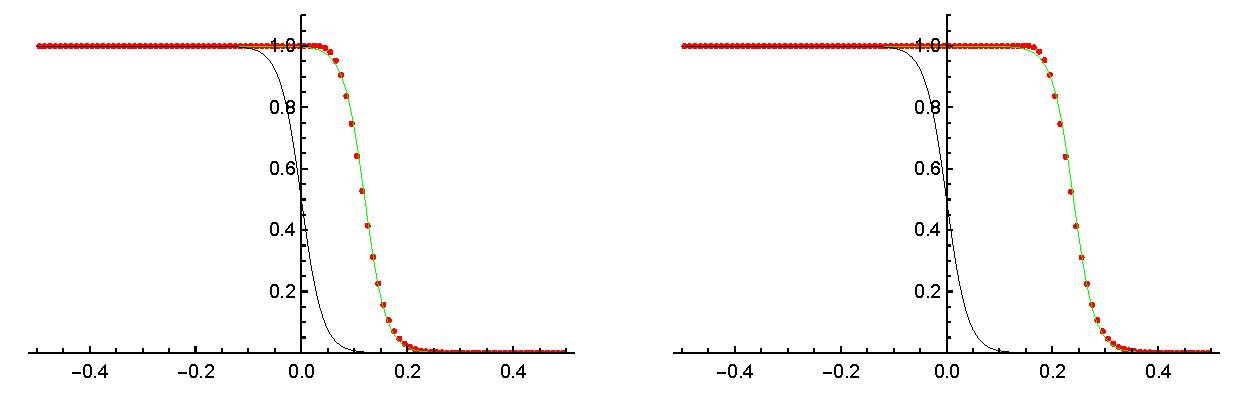
\includegraphics[width=\textwidth]{figures/travel100.pdf}
	\caption{Comparing the $ \mathrm{IIOE} $ scheme with the exact traveling-wave solution {\rm (\ref{travel})} in time $ t=0.24 $ (left) and $ t = 0.48 $ (right), with $ \sigma=0.01 $, $ n=100 $, $ \tau=4h $}
	\label{fig:travel}
\end{figure}

\begin{table}[h!]
	\caption{Report on the $L_2$ errors of $\mathrm{IIOE}$ method for the traveling-wave solution {\rm (\ref{travel})} of the viscous Burgers' equation {\rm (\ref{burg})} with $\sigma = 0.01$, number of nonlinear iterations = 1. }
	\begin{center} \footnotesize
		\begin{tabular}{|c|c|c|c|c|c|}
			\hline  
			$ n $ & $ h $ & $\tau$ & NTS & $L_2(I,L_2)$ & EOC\\
			\hline
			\lower.3ex\hbox{100} & \lower.3ex\hbox{0.01} & \lower.3ex\hbox{0.04} & \lower.3ex\hbox{12} & \lower.3ex\hbox{4.41 $10^{-2}$} &\\
			\hline
			\lower.3ex\hbox{200} & \lower.3ex\hbox{0.005} & \lower.3ex\hbox{0.02} & \lower.3ex\hbox{24} & \lower.3ex\hbox{2.32 $10^{-2}$} & \lower.3ex\hbox{0.93}\\
			\hline
			\lower.3ex\hbox{400} & \lower.3ex\hbox{0.0025} & \lower.3ex\hbox{0.01} & \lower.3ex\hbox{48} & \lower.3ex\hbox{1.18 $10^{-2}$} & \lower.3ex\hbox{0.97}\\
			\hline
			\lower.3ex\hbox{800} & \lower.3ex\hbox{0.00125} & \lower.3ex\hbox{0.005} & \lower.3ex\hbox{96} & \lower.3ex\hbox{5.96 $10^{-3}$} & \lower.3ex\hbox{0.99}\\
			\hline
		\end{tabular}
	\end{center}
	\label{tab:travel_1iter}
\end{table}

\begin{figure}[h!]
	\centering
	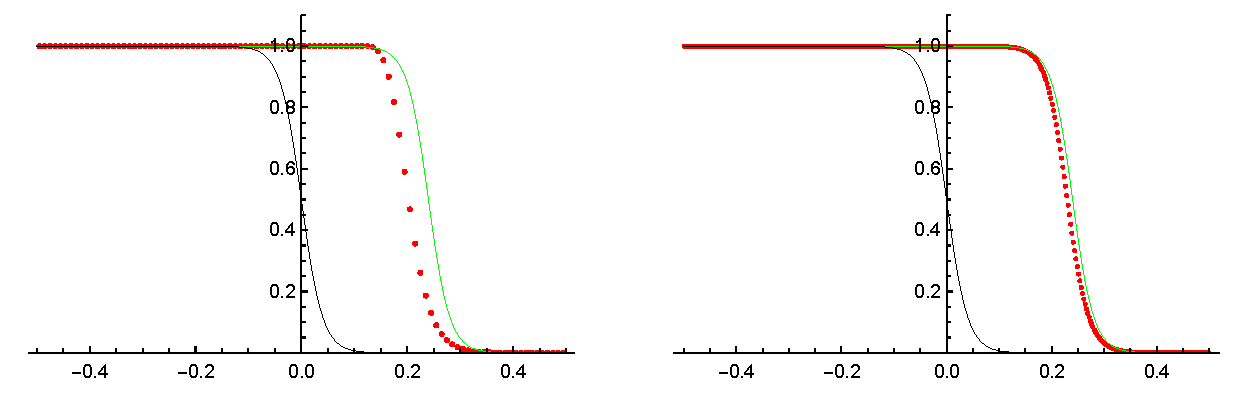
\includegraphics[width=\textwidth]{figures/traveliter}
	\caption{Comparing the $ \mathrm{IIOE} $ scheme with the exact traveling-wave solution {\rm (\ref{travel})} in time $ t=0.48 $, with $ \sigma=0.01 $, $ n=100 $(left), $ n=400 $(right), $ \tau=4h $, $ \textrm{number of nonlinear iterations} = 1 $. We can see that after refining the grid, the propagation speed of the numerical solution is getting closer to the exact speed.}
	\label{fig:travel_iter}
\end{figure}

\begin{table}[h!]
	\caption{Report on the $L_2$ errors of $\mathrm{IIOE}$ method for the traveling-wave solution {\rm (\ref{travel})}  of the viscous Burgers' equation {\rm (\ref{burg})}  with $\sigma = 0.001$. }
	\begin{center} \footnotesize
		\begin{tabular}{|c|c|c|c|c|c|}
			\hline  
			$ n $ & $ h $ & $\tau$ & NTS & $L_2(I,L_2)$ & EOC\\
			\hline
			\lower.3ex\hbox{250} & \lower.3ex\hbox{0.004} & \lower.3ex\hbox{0.016} & \lower.3ex\hbox{30} & \lower.3ex\hbox{2.01 $10^{-2}$} &\\
			\hline
			\lower.3ex\hbox{500} & \lower.3ex\hbox{0.002} & \lower.3ex\hbox{0.08} & \lower.3ex\hbox{60} & \lower.3ex\hbox{6.84 $10^{-3}$} & \lower.3ex\hbox{1.55}\\
			\hline
			\lower.3ex\hbox{1000} & \lower.3ex\hbox{0.001} & \lower.3ex\hbox{0.04} & \lower.3ex\hbox{120} & \lower.3ex\hbox{1.79 $10^{-3}$} & \lower.3ex\hbox{1.94}\\
			\hline
			\lower.3ex\hbox{2000} & \lower.3ex\hbox{0.0005} & \lower.3ex\hbox{0.02} & \lower.3ex\hbox{240} & \lower.3ex\hbox{4.55 $10^{-4}$} & \lower.3ex\hbox{1.97}\\
			\hline
		\end{tabular}
	\end{center}
	\label{tab:travelsig1/1000}
\end{table}

\begin{figure}[h!]
	\centering
	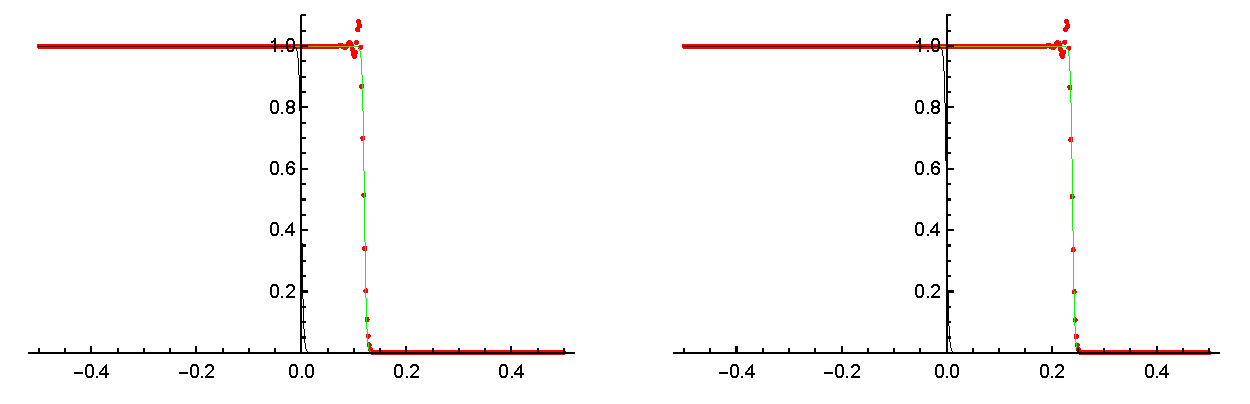
\includegraphics[width=\textwidth]{figures/travelsig0015002448}
	\caption{Comparing the $ \mathrm{IIOE} $ scheme with the exact traveling-wave solution {\rm (\ref{travel})} in time $ t=0.24 $ (left) and $ t = 0.48 $ (right), with $ \sigma=0.001 $, $ n=500 $, $ \tau=4h $. We can observe small nonincreasingly propagating oscillations.}
	\label{fig:travel_sig1/1000_n500}
\end{figure}

\begin{figure}[h!]
	\centering
	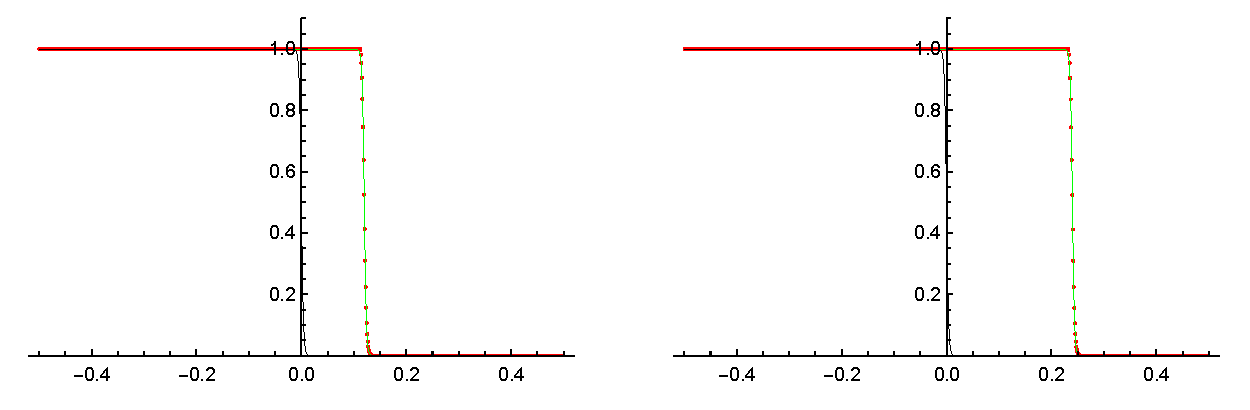
\includegraphics[width=\textwidth]{figures/travelsig0011000024048}
	\caption{Comparing the $ \mathrm{IIOE} $ scheme with the exact traveling-wave solution {\rm (\ref{travel})} in time $ t=0.24 $ (left) and $ t = 0.48 $ (right), with $ \sigma=0.001 $, $ n=1000 $, $ \tau=4h $. On the refined grid the oscillations are gone.}
	\label{fig:travel_sig1/1000_n1000}
\end{figure}
%====================================================================================================================================================
\newpage
\subsection{Rarefaction wave}
The next example can be obtained considering the initial condition
\begin{equation}
	u(0, x)=
	\begin{cases}
		u_l, &x \leq 0,\nonumber\\
		u_r, &x > 0.\nonumber
	\end{cases}
	\label{rareOnR}
\end{equation}
It can be shown that for $ t > 0 $ the exact solution is
\begin{equation}
	u(x,t) = u_{l} + \frac{u_{r}-u_{l}}
	{1 + e^{(u_r - r_l)(x - st) / 2 \sigma}
		\textrm{erfc} \left( \frac{x-u_{l}t}{2\sqrt{\sigma t}} \right) 
		\Big/
		\textrm{erfc} \left( \frac{u_{r}t-x}{2\sqrt{\sigma t}} \right)},
	\label{rare}
\end{equation}
where $ s = (u_l + u_r)\slash 2 $. We chose $ u_l = 0,\,u_r = 1 $, in which case the exact solution corresponds to a rarefaction wave. First, equation (\ref{burg}) is solved by the scheme (\ref{iioe}) on space interval $ (-0.5, 0.5) $ and time interval $ [0.01, 0.41) $ with $ \sigma = 0.01 $. Since the exact solution (\ref{rare}) is defined for $ t>0 $, we decided to initialize the calculation at time 0.01. The time step $ \tau $ was chosen to be equal to $ 4h $ again. The numerical solution is visually compared to the exact solution in Figure \ref{fig:rare}. The errors are presented in Table \ref{tab:rare}.

\begin{table}[h!]
	\caption{Report on the $L_2$ errors of $\mathrm{IIOE}$ method for the rarefaction-wave solution {\rm (\ref{rare})} of the viscous Burgers' equation {\rm (\ref{burg})} with $\sigma = 0.01$. }
	\begin{center} \footnotesize
		\begin{tabular}{|c|c|c|c|c|c|}
			\hline  
			$ n $ & $ h $ & $\tau$ & NTS & $L_2(I,L_2)$ & EOC\\
			\hline
			\lower.3ex\hbox{100} & \lower.3ex\hbox{0.01} & \lower.3ex\hbox{0.04} & \lower.3ex\hbox{10} & \lower.3ex\hbox{5.48 $10^{-3}$} &\\
			\hline
			\lower.3ex\hbox{200} & \lower.3ex\hbox{0.005} & \lower.3ex\hbox{0.02} & \lower.3ex\hbox{20} & \lower.3ex\hbox{1.56 $10^{-3}$} & \lower.3ex\hbox{1.82}\\
			\hline
			\lower.3ex\hbox{400} & \lower.3ex\hbox{0.0025} & \lower.3ex\hbox{0.01} & \lower.3ex\hbox{40} & \lower.3ex\hbox{4.01 $10^{-4}$} & \lower.3ex\hbox{1.96}\\
			\hline
			\lower.3ex\hbox{800} & \lower.3ex\hbox{0.00125} & \lower.3ex\hbox{0.005} & \lower.3ex\hbox{80} & \lower.3ex\hbox{1.00 $10^{-4}$} & \lower.3ex\hbox{2.00}\\
			\hline
		\end{tabular}
	\end{center}
	\label{tab:rare}
\end{table}

\begin{figure}[h!]
	\centering
	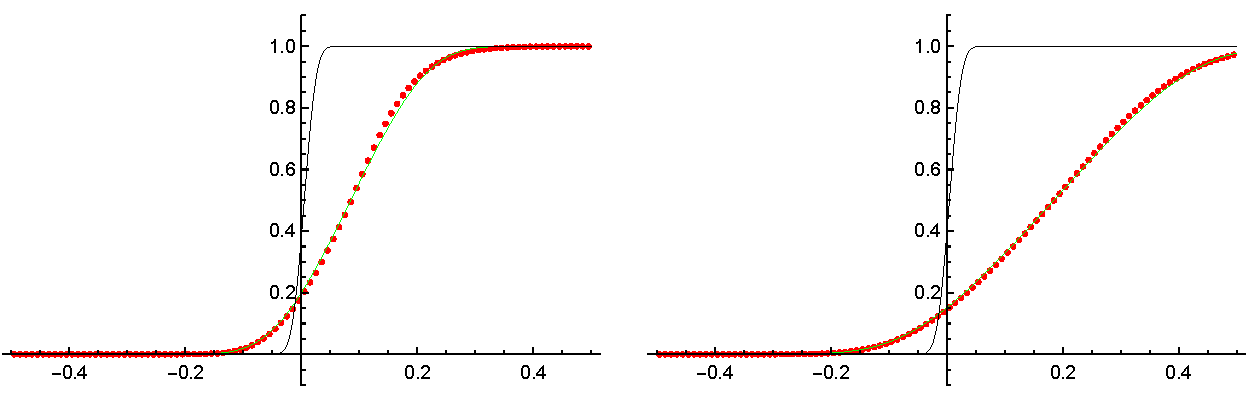
\includegraphics[width=\textwidth]{figures/rare100}
	\caption{Comparing the $\mathrm{IIOE}$ scheme with the exact rarefaction-wave solution {\rm (\ref{rare})} in time $ t=0.17 $ (left) and $ t = 0.41 $ (right), with $ \sigma=0.01 $, $ n=100 $, $ \tau=4h $}
	\label{fig:rare}
\end{figure}

%====================================================================================================================================================

\subsection{Triangular wave}
Another interesting example is the triangular-wave solution
\begin{equation}
	u(x,t)=2 \sqrt{\frac{\sigma}{\pi t}} \frac{e^{-x^{2}/4\sigma t}}{\coth \left(\frac{1}{4\sigma}\right)-\mathrm{erf} \left(\frac{x}{2\sqrt{\sigma t}}\right)},
	\label{triang}
\end{equation}
which is a solution to the problem \eqref{BurgersOnR}, when the initial condition is the delta function $ \delta(x) $ centered at the origin.
In this case the problem (\ref{BurgersOnR}) is solved by the scheme (\ref{iioe}) on space interval $ (-0.5, 1.5) $ and time interval $ (0.01, 0.51) $ with $ \sigma = 0.02 $. Again, the exact solution (\ref{triang}) is defined for $ t > 0 $ so the numerical calculation was initialized at time 0.01. In Table \ref{ttri} we show the errors for refined grids and time step. When the grid size is not sufficiently fine, we can observe oscillations at the peak of the wave \ref{fig:triang-osc}. These oscillations do not grow unboundedly and can be removed by refining the grid as it is shown in Figure \ref{ftri1}.

\begin{table}[ht]
	\caption{Report on the $L_2$ errors of $\mathrm{IIOE}$ method for the triangular-wave solution {\rm (\ref{triang})} of the viscous Burgers' equation {\rm (\ref{burg})} with $\sigma = 0.02$. }
	\begin{center} \footnotesize
		\begin{tabular}{|c|c|c|c|c|c|}
			\hline  
			$n$ & $h$ & $\tau$ & \lower.3ex\hbox{NTS} & \lower.3ex\hbox{$L_2(I,L_2)$} & \lower.3ex\hbox{EOC}\\
			\hline
			\lower.3ex\hbox{100} & \lower.3ex\hbox{0.02} & \lower.3ex\hbox{0.08} & \lower.3ex\hbox{5} & \lower.3ex\hbox{3.07 $10^{-1}$} &\\
			\hline
			\lower.3ex\hbox{200} & \lower.3ex\hbox{0.01} & \lower.3ex\hbox{0.04} & \lower.3ex\hbox{10} & \lower.3ex\hbox{1.30 $10^{-1}$} &\lower.3ex\hbox{1.24}\\
			\hline
			\lower.3ex\hbox{400} & \lower.3ex\hbox{0.005} & \lower.3ex\hbox{0.02} & \lower.3ex\hbox{20} & \lower.3ex\hbox{3.72 $10^{-2}$} &\lower.3ex\hbox{1.81}\\
			\hline
			\lower.3ex\hbox{800} & \lower.3ex\hbox{0.0025} & \lower.3ex\hbox{0.01} & \lower.3ex\hbox{40} & \lower.3ex\hbox{9.02 $10^{-3}$} &\lower.3ex\hbox{2.04}\\
			\hline
		\end{tabular}
	\end{center}
	\label{ttri}
\end{table}

\begin{figure}[h!]
	\centering
	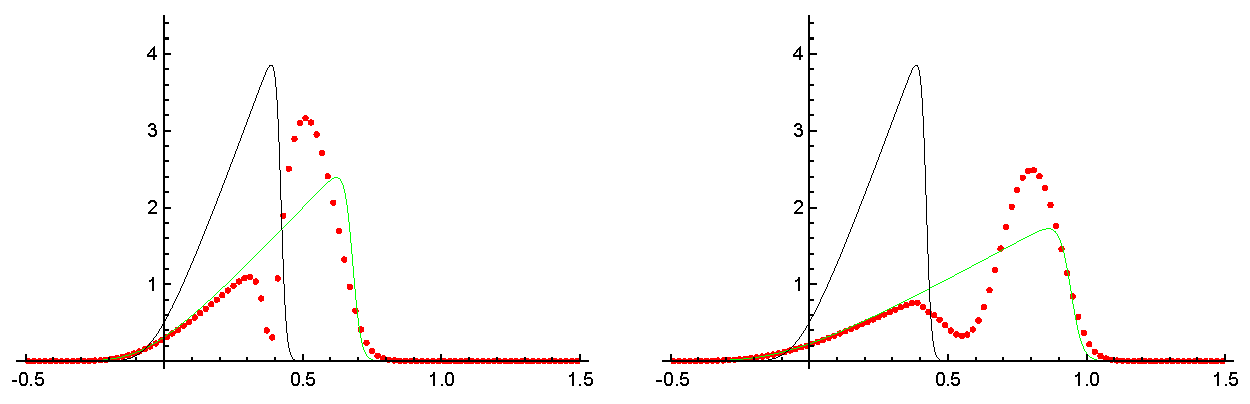
\includegraphics[width=\textwidth]{figures/tri100.pdf}
	\caption{Comparing the $\mathrm{IIOE}$ scheme with the exact traingular wave solution {\rm (\ref{triang})} in time $ t = 0.26 $ (left), $ t = 0.50 $ (right) for $ n=100 $, whith $ \sigma=0.02 $,  $ \tau = 4h $.}
	\label{fig:triang-osc}
\end{figure}

\begin{figure}[h]
	\centering
	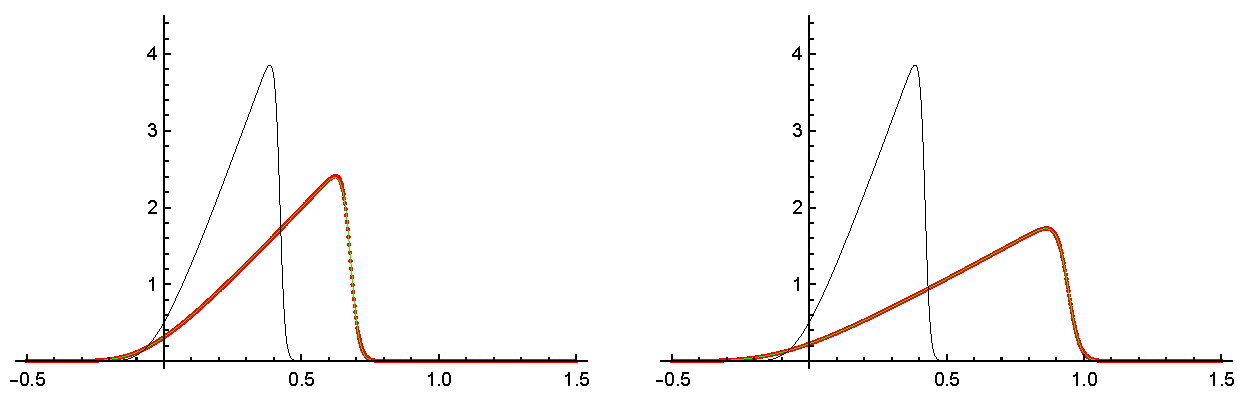
\includegraphics[width=\textwidth]{figures/tri800.pdf}
	\caption{Comparing the $\mathrm{IIOE}$ scheme with the exact traingular wave solution {\rm (\ref{triang})} in time $ t = 0.26 $ (left), $ t = 0.50 $ (right) for $ n=800 $ whith $ \sigma=0.02 $,  $ \tau = 4h $.}
	\label{ftri1}
\end{figure}

%====================================================================================================================================================

\subsection{Trigonometric solution}
Our last example is the trigonometric solution
\begin{equation}
	u(x,t)=\frac{2\sigma b \pi \sin{\pi x}}{ae^{\sigma \pi^{2}t}+b\cos \pi x },
	\label{trig}
\end{equation}
where $ a \textrm{ and } b $ are constants, $ a > b $. This solution can be obtained transforming a separable solution to the linear heat equation. We The errors are reported in Table \ref{ttrig}. A visual comparison of the numerical results with the exact solution is presented in Figure \ref{ftrig}.

\begin{table}[h!]
	\caption{Report on the $L_2$ errors of $\mathrm{IIOE}$ method for the trigonometric solution {\rm (\ref{trig})} of the viscous Burgers' equation {\rm (\ref{burg})} with $\sigma = 0.01$. }
	\begin{center} \footnotesize
		\begin{tabular}{|c|c|c|c|c|c|}
			\hline
			$n$ & $h$& $\tau$ & NTS & $L_2(I,L_2)$ & EOC\\
			\hline
			\lower.3ex\hbox{100} & \lower.3ex\hbox{0.02} & \lower.3ex\hbox{0.08} & \lower.3ex\hbox{15} & \lower.3ex\hbox{1.66 $10^{-2}$} &\\
			\hline
			\lower.3ex\hbox{200} & \lower.3ex\hbox{0.01} & \lower.3ex\hbox{0.04} & \lower.3ex\hbox{30} & \lower.3ex\hbox{3.18 $10^{-3}$} &\lower.3ex\hbox{2.38}\\
			\hline
			\lower.3ex\hbox{400} & \lower.3ex\hbox{0.005} & \lower.3ex\hbox{0.02} & \lower.3ex\hbox{60} & \lower.3ex\hbox{5.30 $10^{-4}$} &\lower.3ex\hbox{2.58}\\
			\hline
			\lower.3ex\hbox{800} & \lower.3ex\hbox{0.0025} & \lower.3ex\hbox{0.01} & \lower.3ex\hbox{120} & \lower.3ex\hbox{1.00 $10^{-4}$} &\lower.3ex\hbox{2.41}\\
			\hline
		\end{tabular}
	\end{center}
	\label{ttrig}
\end{table}

\begin{figure}[h!] 
	\centering
	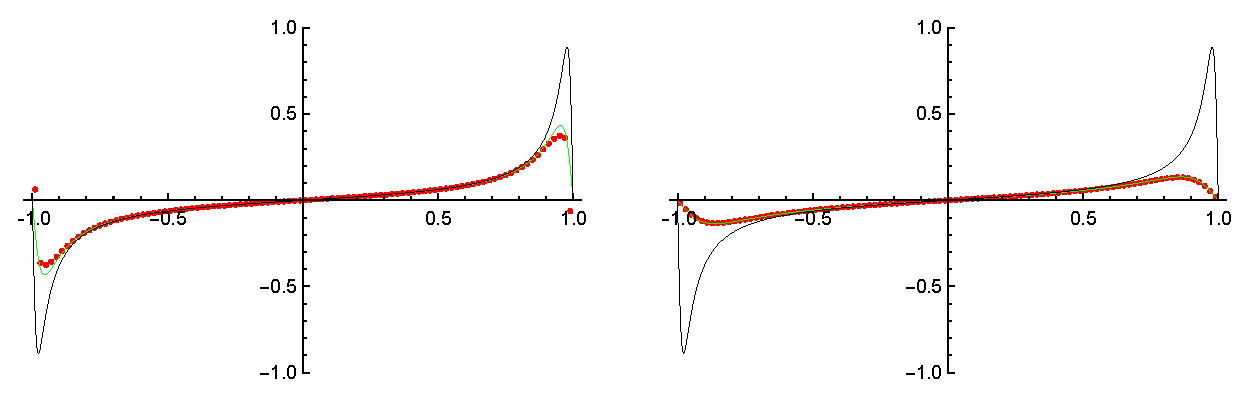
\includegraphics[width=\textwidth]{figures/trig100}
	\caption{Comparing the $\mathrm{IIOE}$ scheme with the exact trigonometric solution {\rm (\ref{trig})} in time $ t = 0.08 $ (left) and $ t = 0.96 $ (right) for $ n=100 $, with $ \sigma=0.01 $, $ b=1 $, $ a=1.0025 $, $ \tau = 4h $.}
	\label{ftrig} 
\end{figure} 

%====================================================================================================================================================
\newpage
\section{Traffic flow}
In this section we solve 
\begin{equation}
	\rho_t + (1 - 2\rho)\rho_x = D \rho_{xx},\quad x\in \mathbb{R},\, t > 0.
	\label{trafficonR}
\end{equation}
As discussed earlier, by making certain assumptions about the flux function, we can transform the the solutions of Burgers' equation \eqref{BurgersOnR} to obtain a solution for the density of the cars in the traffic flow problem (\ref{trafficonR}). Below we give an interpretation of the traveling-wave and the rarefaction-wave solution in a traffic flow context.

\subsection{Traveling wave}
A traveling wave can form in a traffic, when incoming cars are approaching a congestion or a line of cars staying behind a red light waiting for turning to green. In the congestion, the density $ \rho_r = 1 $, which means bumper to bumper traffic. The density of the incoming traffic was chosen to be $ \rho_r = 0.1 $, which means that there is one car/10 car lengths.

The exact solution for the density was obtained as follows: considering the densities $ \rho_l = 0,\,\rho_l = 1 $ and using the relationship \eqref{u-ro} we can calculate $ u_l = 0.8$ and $ u_r = -1 $ for the traveling wave solution \eqref{travel} of the Burgers' equation. Then using the relationship (\ref{ro-u}) we obtain the solution for the density. This solution for the traffic density $ \rho $ was compared to the numerical solution using the IIOE scheme (\ref{iioe}). The errors are documented in Table \ref{tab:density_travel_sig1/1000}. The solution for $ \sigma = 0.01 $ is presented in Figure \ref{fig:traffic_travel}.
\begin{table}[h!]
	\caption{Report on the $L_2$ errors of $\mathrm{IIOE}$ method for the traffic flow problem {\rm (\ref{traffic})} with $\sigma = 0.01$. }
	\begin{center} \footnotesize
		\begin{tabular}{|c|c|c|c|c|c|}
			\hline  
			$ n $ & $ h $ & $\tau$ & NTS & $L_2(I,L_2)$ & EOC\\
			\hline
			\lower.3ex\hbox{100} & \lower.3ex\hbox{0.01} & \lower.3ex\hbox{0.04} & \lower.3ex\hbox{12} & \lower.3ex\hbox{9.82 $10^{-4}$} &\\
			\hline
			\lower.3ex\hbox{200} & \lower.3ex\hbox{0.005} & \lower.3ex\hbox{0.02} & \lower.3ex\hbox{24} & \lower.3ex\hbox{2.36 $10^{-4}$} & \lower.3ex\hbox{2.05}\\
			\hline
			\lower.3ex\hbox{400} & \lower.3ex\hbox{0.0025} & \lower.3ex\hbox{0.01} & \lower.3ex\hbox{48} & \lower.3ex\hbox{5.94 $10^{-5}$} & \lower.3ex\hbox{1.99}\\
			\hline
			\lower.3ex\hbox{800} & \lower.3ex\hbox{0.00125} & \lower.3ex\hbox{0.005} & \lower.3ex\hbox{96} & \lower.3ex\hbox{1.53 $10^{-5}$} & \lower.3ex\hbox{1.96}\\
			\hline
		\end{tabular}
	\end{center}
	\label{tab:density_travel_sig1/1000}
\end{table}
\begin{figure}[h!]
	\centering
	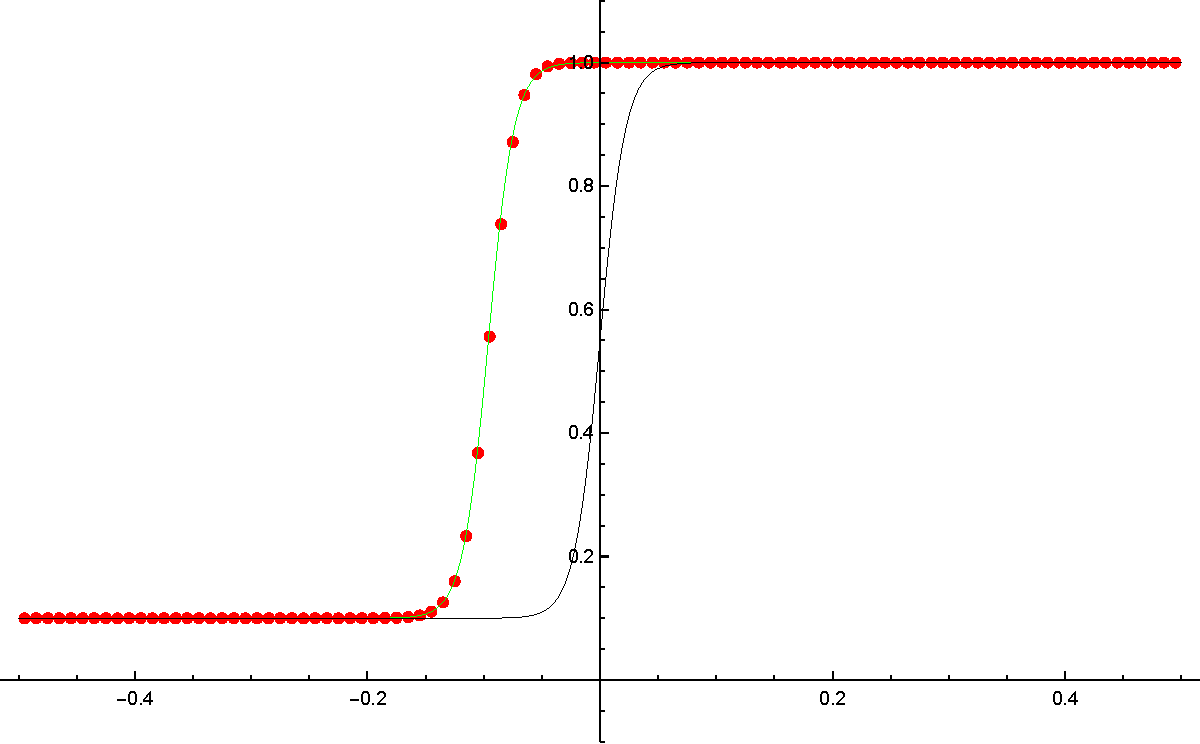
\includegraphics[width=\textwidth]{figures/trafficTravel100t.96}
	\caption{Cars from left with traffic density $ \rho_l = 0.1 $ are approaching the congested region with $ \rho_r = 1 $. This would happen, for example, when cars are staying behind a red light. 
	The blue line is the initial condition for the numerical computation, the red dots are the values computed by the IIOE scheme. The green line is the exact solution obtained by transforming the traveling-wave solution {\rm (\ref{travel})} of the Burgers' equation {\rm (\ref{burg})}(left) using {\rm (\ref{ro-u})}. The results of the numerical solution are shown at time $ t = 0.96 $, for $ n = 100 $, $ \tau = 4h $, $ \sigma = 0.01 $.
	}
	\label{fig:traffic_travel}
\end{figure}

%====================================================================================================================================================
\newpage
\subsection{Rarefaction wave}
We also interpret the rarefaction wave solution in a traffic flow context. Imagine that the road is divided into two parts by the traffic light positioned at the origin. Cars to the left are staying behind the red light for $ t<0 $, so the density $ \rho_l = 1 $ there. On the right there is an empty road, $ \rho_r = 0 $. At time $ t = 0 $ the light turns green. This corresponds to the initial condition for a traffic light positioned at $ x = 0 $
\begin{equation}
	\rho(0,x) =
	\begin{cases}
		1, &x\leq 0,\nonumber\\
		0, &x>0,\nonumber
	\end{cases}
\end{equation}
Right after the light turned green, the cars start to leave, the traffic rarifies. The exact solution for the density in (\ref{trafficonR}) was obtained the same way as in our previous example. First, considering the values $ \rho_l = 1 $, $ \rho_r = 0 $ we calculate the corresponding values $ u_l = -1 $, $ u_r = 1 $ according to (\ref{u-ro}) for the rarefaction wave solution of the Burgers' equation. Then substituting the exact solution (\ref{rare}) to (\ref{ro-u}) we get the density function. The numerical solution for the density by the IIOE scheme (\ref{iioe}) is presented for $ \sigma = 0.01 $ in Figure \ref{fig:traffic_rare}.

\begin{figure}[h!]
	\centering
	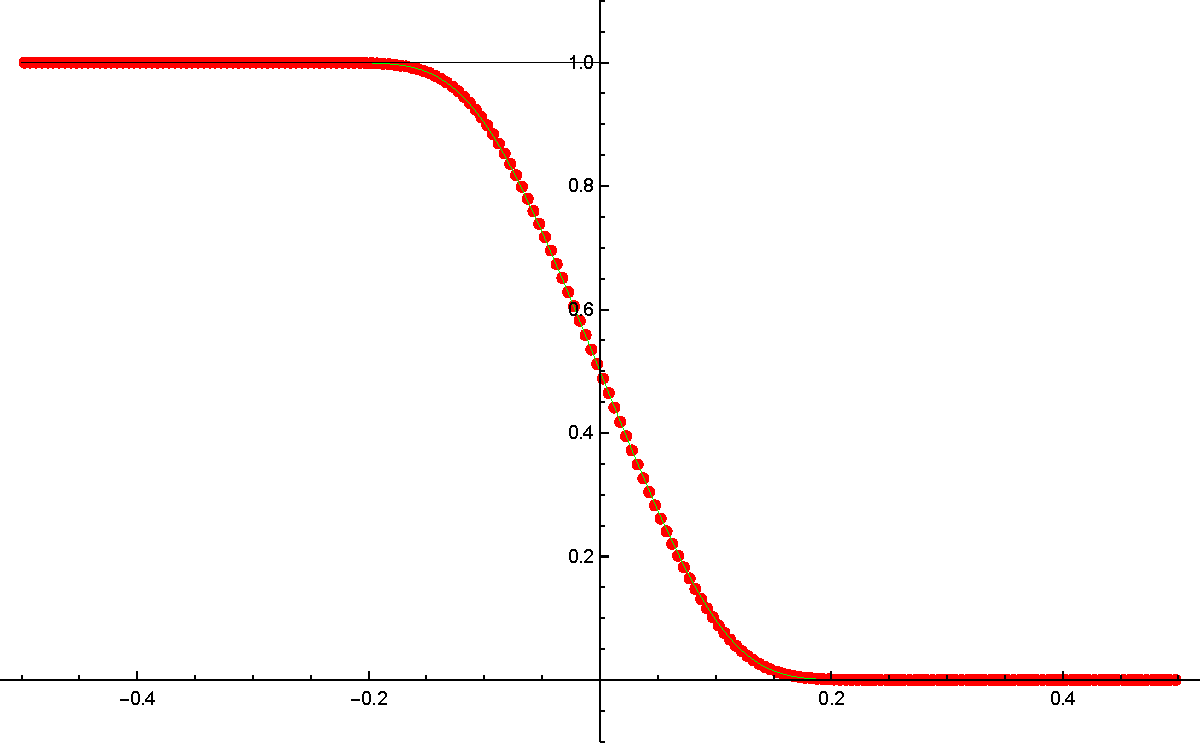
\includegraphics[width=\textwidth]{figures/trafficRare1}
	\caption{At $ t<0 $ cars to the left of the origin are staying behind a red light, the density $ \rho_l = 1 $. To the right there is an empty road, $ \rho_r = 0 $. At time $ t = 0 $ the traffic light at the origin turns green and cars start to leave. The black line is the initial condition. At time $ t = 0.08 $ the exact solution(green) is compared to the values obtained by numerical computation(red) for $ n = 100 $, $ \tau = h $, $ \sigma = 0.01 $. The exact solution for the density of cars was obtained by transforming the rarefaction-wave solution {\rm (\ref{rare})} of the Burgers' equation {\rm (\ref{BurgersOnR})} using {\rm (\ref{ro-u})}.}
	\label{fig:traffic_rare}
\end{figure}
%====================================================================================================================================================

\chapter{Thesis objectives}
\chaptermark{Thesis objectives}
In the future we plan to perform the following tasks:
\begin{itemize}
	\item Test the scheme on other models of traffic flow
	\item Using the scheme for computing traffic flow on networks
	\item Stabilization of the method for problems whose solutions are tending to develop shocks
\end{itemize}
%====================================================================================================================================================

\begin{thebibliography}{9}
	\bibitem{bateman} {\sc H. Bateman},
	{\em Some recent researches on the motion of fluids}, Monthly Weather Rev. 43 (1915), 63-170.
	
	\bibitem{batchelor} {\sc G. K. Batchelor}
	{\em An introduction to fluid dynamics}, Cambridge University Press, Cambridge, 1967.
	
	\bibitem{wageningen} {\sc F. van Wageningen-Kessels, H. van Lint, K. Vuik, S. Hoogendoorn}
	{\em Genealogy of traffic flow models}, EURO Journal on Transportation and Logistics, 4(4):445-473, 12 2015.
	
	\bibitem{burgers} {\sc J. M. Burgers},
	{\em A mathematical model illustrating the theory of turbulence}, Adv. Appl. Mech. 1 (1948), 171-199.
	
	\bibitem{lev} {\sc R.J. LeVeque}, 
	{\em Finite Volume Methods for Hyperbolic Problems}, Cambridge Texts in Applied Mathematics. Cambridge University Press, 2002.
	
	\bibitem{olv} {\sc P. J. Olver}, 
	{\em Introduction to Partial Differential Equations}, Undergraduate Texts in Mathematics. Springer, New York, 2014.
	
	\bibitem{iioe0} {\sc K. Mikula, M. Ohlberger}, 
	{\em A new Inflow-Implicit/Outflow-Explicit Finite Volume Method for Solving Variable Velocity Advection Equations}, Preprint 01/10 - N, Angewandte Mathematik und Informatik, Universitaet M\"{u}nster, June 2010
	
	\bibitem{iioe1} {\sc K. Mikula, M. Ohlberger},
	{\em Inflow-Implicit/Outflow-Explicit Scheme for Solving Advection Equations}, in Finite Volumes in Complex Applications VI, Problems \& Perspectives, Eds.J.Fo\u{r}t et al. (Proceedings of the Sixth International Conference on Finite Volumes in Complex Applications, Prague, June 6-10, 2011), Springer Verlag, 2011, pp. 683-692.
	
	
	\bibitem{iioe2} {\sc K. Mikula, M. Ohlberger, J.Urban}, 
	{\em Inflow-Implicit/Outflow-Explicit finite volume methods for solving advection equations}, Applied Numerical Mathematics, Vol. 85 (2014) pp. 16-37
	
	\bibitem{greenshields} {\sc B. N. Greenshields},
	{\em A study of traffic capacity}, In Proceedings of the 14th Annual Meeting of the Highway Research Board, 1934, pp. 448-474.
	
	\bibitem{lighthillwitham} {\sc M. J. Lighthill and G. B. Whitham},
	{\em On kinematic waves II: A theory of traffic flow on long crowded roads}, Proc. Roy. Soc. London Ser. A, (1955), pp. 317-345.
	
	\bibitem{richards} {\sc P. I. Richards},
	{\em Shock waves on highways}, Oper. Res., 4 (1956), pp. 42-51.
	
	\bibitem{whitham} {\sc G. B. Whitham}, 
	{\em Linear and Nonlinear Waves}, Wiley-Interscience, 1974.
	
	\bibitem{kachroo-sastry} {\sc P. Kachroo, S. Sastry},
	{\em Traffic flow theory: Mathematical Framework.} University of California Berkeley
	
\end{thebibliography} 
\end{document}
